\newpage
\Question{Backprop: \emph{Adapted from Fall 2015 Final Exam}}

Suppose we have a neural network that takes in $P = 2$ input features, has $H = 4$ hidden units, and $N = 1$ output.
\begin{figure}[h!]
\begin{center}
  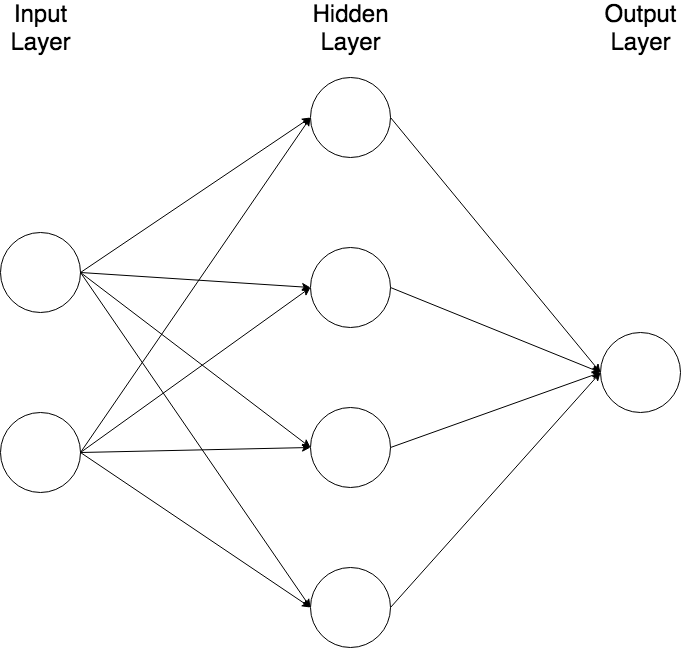
\includegraphics[width=5in]{src/problems/nn/small_neural_net.png}
  \caption{Unlabeled neural network as described above.}
\end{center}
\end{figure}

$f(x)$ is the activation function in the hidden layer, and $g(x)$ is the activation function in the output layer.

Let's define some notation! \\
$x\in \mathcal{R}^{P}$ is a feature vector\\
$s^h_j = \sum_{i=1}^{P} V_{i, j}x_i$ are inputs to the hidden layer \\
$h_j = f(s^h_j)$\\
$s^o_k = \sum_{j=1}^{H} W_{j, k}h_j$ are inputs to the output layer\\
$z_k = g(s^o_k)$ \\
$V \in \mathcal{R}^{H\times P}$ are weights between input layer and hidden layer\\
$W \in \mathcal{R}^{N\times H}$ are weights between hidden layer and output layer\\

\begin{Parts}

\Part
On the diagram provided, label each of the pieces of notation defined above in their appropriate places.
Focus on understanding the role of each variable in defining your neural net;
don't worry too much about the exact details of how to annotate the diagram.

Now, draw in a bias term to both the input layer and the hidden layer and connect it appropriately with the other nodes.

\begin{solution}
The filled-in neural net with bias terms looks like this:
\begin{center}
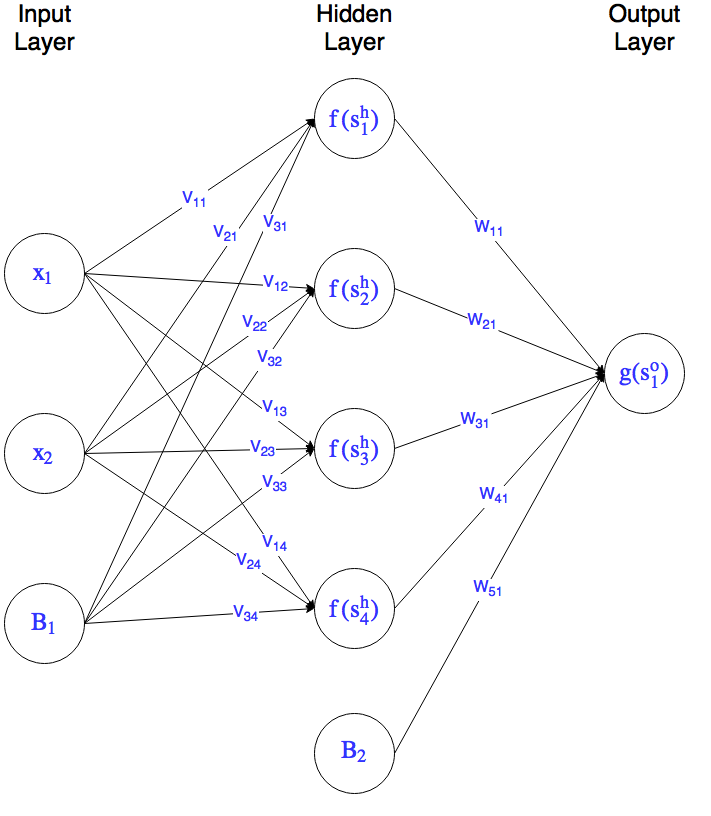
\includegraphics[width=5in]{src/problems/nn/small_neural_net_soln.png}
\end{center}
Here, $x_i$ represents the $i^{th}$ input neuron, also known as the $i^{th}$ feature of our input vector. $B_i$ is the bias neuron for the $i^{th}$ layer. $V_{ij}$ is the weight connecting the $i^{th}$ input neuron with the $j^{th}$ hidden neuron. Remember that $s_i^h$ is the input to the $i^{th}$ hidden neuron, where $s_j^h=\sum_{i=1}^{3}V_{ij}*x_i$. This input is put through the hidden layer's activation function $f(x)$ to get the value of that node. Likewise, $W_{ij}$ is the weight connecting the $i^{th}$ hidden neuron with the $j^{th}$ output neuron, and $s_j^o=\sum_{i=1}^{5}V_{ij}*f(s^h_i)$. Finally, this is passed through the output layer's activation function $g(x)$ to get our final output.


\end{solution}

\Part
Suppose you want to include a bias term in both the input layer and hidden layer,
how many weights will be trained in total now? What will be the dimensions of our weight matrices $V$ and $W$ if we include these bias terms?
What if we had $P=p$ input features, $l$ hidden layers each with $H=h$ hidden units, $N=n$ outputs, and bias terms in both the input and hidden layers?

\begin{solution}
With bias terms:
$$(2+1)\times 4 + (4+1)\times1$$

Our weight matrices will then have the dimensions:
$$V \in \mathcal{R}^{4 \times (2+1)} \text{ and } W \in \mathcal{R}^{1 \times (4+1)}$$
since $V$ contains the weights between the input layer (with bias) and hidden layer,
and $W$ contains the weights between the hidden layer (with bias) and output layer.\\

Generalized neural network with bias terms:
$$(p+1)h + \max(0,l-1)(h+1)h+(h+1)n$$
which follows the pattern of counting weights by taking the number of nodes in the layer before plus one for for the bias "node"
and multiplying it by the number of nodes in the next layer (because our neural net is fully connected), doing this for every pair of adjacent layers.
\end{solution}

\Part
Use the chain rule to expand the following partial derivatives (no need to find the actual derivatives themselves): \\
    \begin{flalign*}
        &\frac{\partial L}{\partial W_{j,k}} = & \\
        &\frac{\partial L}{\partial V_{i,j}} = \\
    \end{flalign*}
\begin{solution}
Back propagation is just a nice term for calculating derivatives using the chain rule. \textbf{The key to using the chain rule in neural networks is to know which variables are related and which variables are independent of each other}. Since $W_{jk}$ is the weight between neuron $h_j$ in the hidden layer and neuron $z_k$ in the output layer, it's important to see $W_{jk}$ and $z_k$ are related while $W_{jk}$ and $z_{k+1}$ are not. By the same reason,
\begin{align*}
     \frac{\partial L}{\partial W_{j, k}} &= \frac{\partial L}{\partial z_k} \frac{\partial z_k}{\partial s^o_k} \frac{\partial s^o_k}{\partial W_{j, k}}
\end{align*}
In the same way, $V_{ij}$ is the weight between each neuron $x_i$ in the input layer and each neuron $h_j$ in the hidden layer and each $h_j$ affects all the neurons in the output layer. Thus when deriving $\frac{\partial L}{\partial V_{ij}}$, we should apply the chain rule over all output neurons and over only a single neuron $h_j$ in the hidden layer.
\begin{align*}
    \frac{\partial L}{\partial V_{i, j}} &= \sum_{k=1}^N \frac{\partial L}{\partial z_k} \cdot \frac{\partial z_k}{\partial s^o_k} \cdot \frac{\partial s^o_k}{\partial h_j} \cdot \frac{\partial h_j}{\partial s^h_j} \cdot \frac{\partial s^h_j}{\partial V_{i, j}}
\end{align*}
\end{solution}

\Part
The softmax function, or normalized exponential function, is a generalization of the logistic function to handle multiclass classification. The softmax function ``squashes" a N-dimensional vector $s$ of arbitrary real values to a K-dimensional vector $\sigma(s)$ of real values in the range [0, 1] that add up to 1. The $i$-th value corresponds to the probability that the output is class $i$. The function is given by the following:
$$ \sigma(s_j) = \dfrac{e^{s_j}}{\sum_{k=1}^N e^{s_k}} \qquad
\text{ for } j = 1 ... N $$

The cross entropy error is commonly paired with softmax activation in the output layer and is defined as:
$$ L(z) = \sum_{k=1}^N y_k \ln (z_k)$$
Now, let $g(x)$ be the softmax function and let our loss function be the cross entropy loss. Calculate the partial derivative of $L$ with respect to $W_{i,j}$. (Note: For part (c), you were not required to calculate the actual derivative. For this part, you must do so.)

\begin{solution}
Notice, that our solution from part (c) is no longer accurate because we had assumed $z_k$ did not depend on $W_{i,j}$ if $k \neq j$. However, by the mechanics of the softmax function, that is no longer true, so we have to sum over all $z_k$.
$$ \dfrac{\partial L}{\partial W_{i,j}} = \sum_{k=1}^N \dfrac{\partial L}{\partial z_k} \dfrac{\partial z_k}{\partial s_j} \dfrac{\partial s_j}{\partial W_{i,j}}$$
$$ \dfrac{\partial L}{\partial z_k} = -\dfrac{y_k}{z_k}$$
\[
  \dfrac{\partial z_k}{\partial s_j} =
  \begin{cases}
  z_k(1-z_k)                         & \text{if $i=k$} \\
  -z_i z_k                           & \text{if $i\neq k$}
  \end{cases}
\]
$$ \dfrac{\partial s_j}{\partial W_{i,j}} = h_i $$
\begin{align*}
\dfrac{\partial L}{\partial W_{i,j}}
&= \sum_{k=1}^N \dfrac{\partial L}{\partial z_k} \dfrac{\partial z_k}{\partial s_j} \dfrac{\partial s_j}{\partial W_{i,j}}\\
&= \dfrac{\partial s_j}{\partial W_{i,j}} (\dfrac{\partial L}{\partial z_j} \dfrac{\partial z_j}{\partial s_j} + \sum_{k \neq j}^N \dfrac{\partial L}{\partial z_k} \dfrac{\partial z_k}{\partial s_j})\\
&= \dfrac{\partial s_j}{\partial W_{i,j}} (-\dfrac{y_j}{z_j} z_j(1-z_j) + \sum_{k \neq j}^N -\dfrac{y_k}{z_k} (-z_j z_k))\\
&= \dfrac{\partial s_j}{\partial W_{i,j}} (-y_j (1-z_j) + \sum_{k \neq j}^N  y_k z_j )\\
&= \dfrac{\partial s_j}{\partial W_{i,j}} (-y_j + y_j z_j + \sum_{k \neq j}^N  y_k z_j )\\
&= \dfrac{\partial s_j}{\partial W_{i,j}} (-y_j + \sum_{k = 1}^N  y_k z_j )\\
&= \dfrac{\partial s_j}{\partial W_{i,j}} (-y_j + z_j \sum_{k = 1}^N  y_k  )\\
&= \dfrac{\partial s_j}{\partial W_{i,j}} (-y_j + z_j)\\
&= h_i (-y_j + z_j)\\
\end{align*}

\end{solution}
\end{Parts}

\newpage
